\documentclass[12pt]{article}
\usepackage[francais]{babel}
\usepackage[latin1]{inputenc}
\usepackage[T1]{fontenc} % pour pouvoir utiliser des caract�res accentu�s dans le fichier source .tex
\usepackage{graphicx}
\usepackage{amssymb}
\textwidth 16cm % largeur du texte
\textheight 25.5cm % hauteur du texte
\voffset -2.5cm % offset vertical
\hoffset -2.cm % offset horizontal
\renewcommand{\refname}{R\'ef\'erences en fran\c{c}ais} % pour que le titre de la bibliographie soit ``Reference en francais'' avec les accents et la c\'edille.
%\usepackage{vmargin}
\usepackage{amsmath}
%\usepackage{amssymb}
%\usepackage{latexsym}

\begin{document}
$$
X_n \xrightarrow[\mathbb{P} \rightarrow \infty]{}  X
$$

$$
X_n \xrightarrow{n \rightarrow \infty} X
$$

$\xrightarrow[\text{en dessous}]{\text{au dessus}}$

\begin{center}
{\Huge Un texte centr\'e en mode Huge}
\end{center}
\vskip .8cm % un espace vertical de .8cm
\section{Une premi\`ere section}
Le texte de cette section
\subsection{Sous-section de la section une}
Le texte de la sous-section
\subsection{Une autre sous-section}
Avec une \'equation num\'erot\'ee \`a droite :
\begin{equation}
(A*B)_{ij} = \sum_{k=1}^{n} a_{ik} b_{kj}
\end{equation}
\begin{equation}
(A*B)_{ij} = \sum_{k=1}^{n} a_{ik} b_{kj}
\end{equation}

\section{Une deuxi\`eme section}
Le texte associ\'e et une r\'ef\'erence \`a \cite{monarticle}

\subsection{Une sous-section pour le graphique Figure \ref{Numerodefigure}}
On ins\`ere un graphique centr\'e et encadr\'e, avec une l\'egende et un num\'ero de figure gr\^ace aux commandes $\backslash$fbox (qui encadre), $\backslash$figure,$\backslash$includegraphics  et $\backslash$caption.

\begin{figure}[h]
\begin{center}
\fbox{
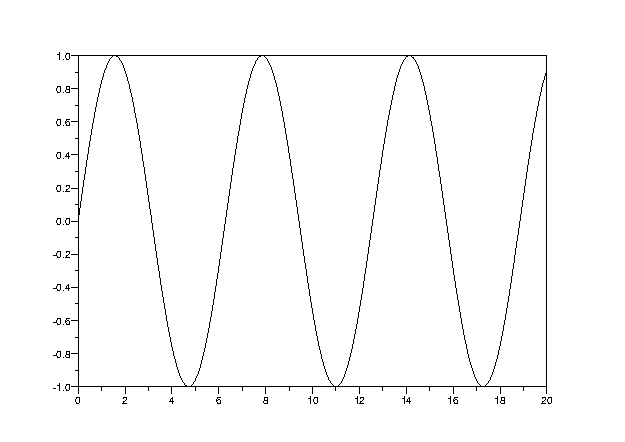
\includegraphics[width=5cm]{graphique.pdf}
}
\caption{\label{Numerodefigure} Ceci est la l\'egende}
\end{center}
\end{figure}


% La bibliographie
\begin{thebibliography}{99}
\bibitem{monarticle} Les auteurs, le titre de l'ouvrage, l'\'editeur
l'ann\'ee de parution
\end{thebibliography}
\end{document}
